\title{Exercise 9}
\author{
        Philip Flyvholm - phif@itu.dk
}
\date{\today}

\documentclass[12pt]{article}
\usepackage{graphicx}
\graphicspath{ {./images/} }
\begin{document}
\maketitle
\begin{figure}[h]
    \centering
    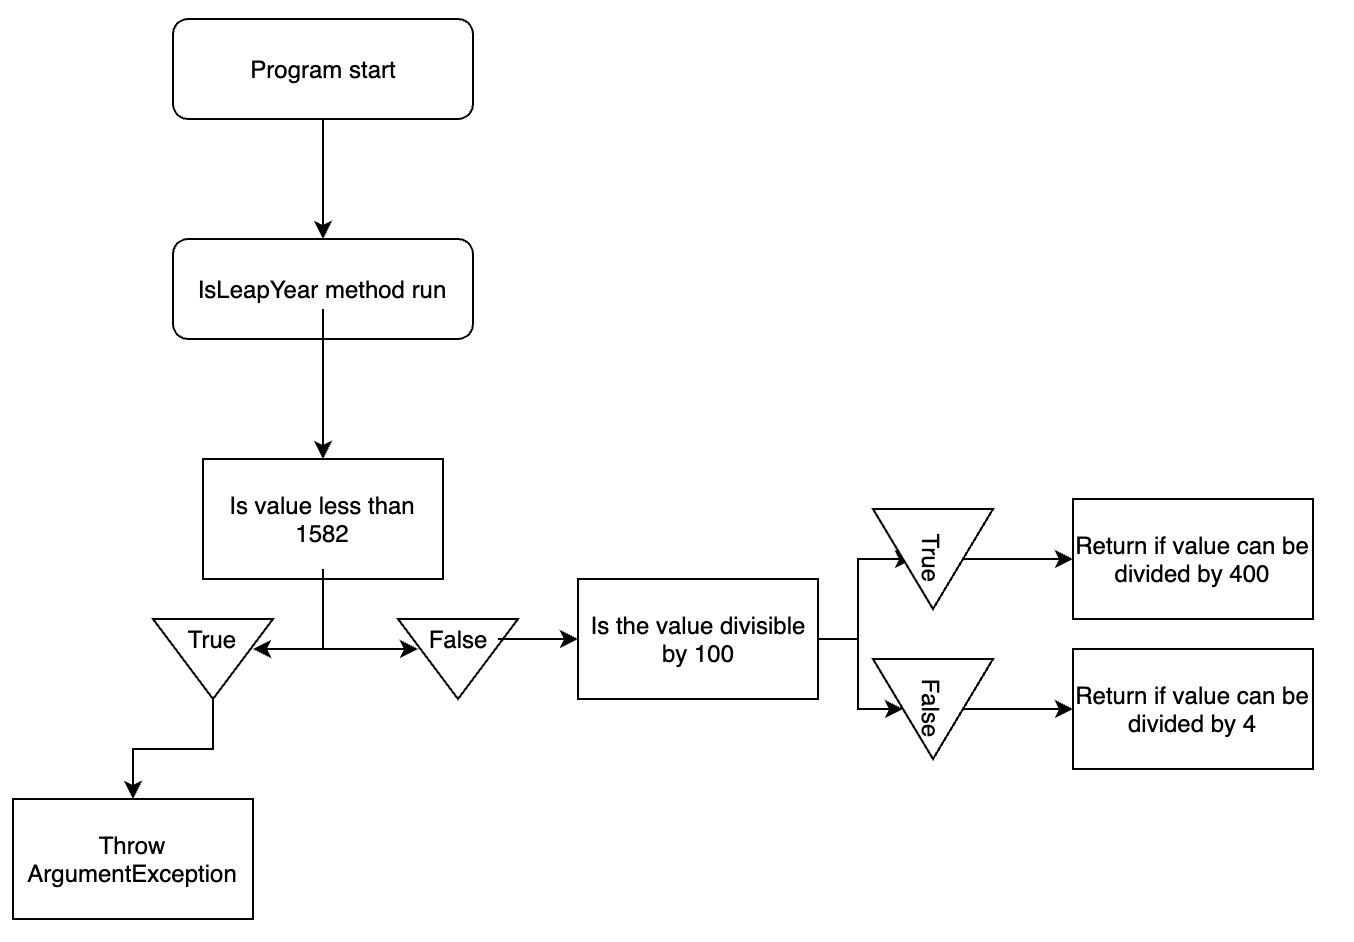
\includegraphics[width=0.8\textwidth]{images/UML_chart.png}
    \caption{Diagram of the IsLeapYear algorithm}
\end{figure}

\paragraph{The method IsLeapYear takes an int parameter referenced as year. The method will throw an ArgumentException if the year is less then 1582. The method returns a boolean, which is true if the given year is a leap year.\\\\
When the method is called then it checks if the given value is less than 1582. If this is true then it throws the ArgumentException. If it is false then it checks if the value is divisible by 100. When this condition is true the method will return true if the value can be devided by 400. If the condition is not met then the method will return true if the value is divisible with 4, otherwise it will return false.}
\end{document}